%\documentclass[11pt, a4paper]{report}
\documentclass[11pt, a4paper]{article}
%report for large text, article for small text
%for hyperlink
\usepackage[dvipdfmx]{hyperref}
%for inserting figure
\usepackage[dvipdfmx]{graphicx}
%https://www.meganii.com/blog/2010/01/14/1263458561/
\setlength\intextsep{0pt}
\setlength\textfloatsep{0pt}
\setlength\floatsep{0pt}
\setlength\abovecaptionskip{0pt}

\title{Experimental Design in Computer  Science \\ \href{https://manaba.tsukuba.ac.jp/ct/course_1910418_report_1960312}{\underline{week1 report}}}

%https://www.isc.meiji.ac.jp/~mizutani/tex/link_slide/hyperlink.html
%\author{Name: Rintaro Sato \and Student ID: 202120597}
\author{Rintaro Sato \\ ID: 202120597}
\date{\today}
%\break
%\newline

\begin{document}
%output title
\maketitle


%\chapter{Choose a scientific question to answer}
%\part{Choose a scientific question to answer}
%\section{Choose a scientific question to answer}
%\subsection{the objective of the experiment}
\centerline{GitHub repo is available at}
\centerline{\underline{\url{https://github.com/rintarooo/time_cpp_python}}}

\noindent
\parindent = 0pt

\section{Objective}
My research interest is Computer Vision and Image Processing, so I use C++ as a one of the my main language. Also, I work on the research in the field where Machine Learning is applied to Computer Vision so Python is also the language I often use for coding.\\

One thing I am curious about these coding languages when I code. Which one is faster? And how fast? I would like to compare them in terms of runtime speed; C++ vs Python.\\

Since Python is an interpreted language while C++ is a compiled language, everyone assumes that C++ would be much faster. However, No one has conducted an experiment comparing program's execution time between these languages in details.\\

My hypothesis is C++ runs 5 times faster than running in Python on average. This report aims to compare their running time.

%\section{Design an Experiment to gather data to answer that question}
\section{Data Collection}
\subsection{Method}
In this report, I implemented the following algorithm related to basic mathematical operation and Computer Vision/Machine Learning in both Python and C++ in order to compare them.\\

- Fibonacci sequence with recursive function 

%- Dijkstra's algorithm for Single Short Path

%- Filtering in Image Processing

- Support Vector Machine(SVM) with OpenCV library\\

OpenCV is a popular library for Computer Vision. I executed the exact same program 30 times in each language, measured the time of each program's execution and then took the average of 30 execution times to compare their running speed.

\subsection{Precaution}
I exactly implemented the same program and the same algorithm order in both languages. I make sure outputs and return values of functions do not differ between Python and C++ programs.\\

In order to get precise execution time, I used the command \href{https://en.wikipedia.org/wiki/Time_(Unix)}{\underline{time}} to time a program's execution. Python and C++ has its own module to time running program but I applied the same method to time for fairness. This \href{https://linuxize.com/post/linux-time-command/}{\underline{time}} command has 2 types, shell built-in command and GNU command. I used former type, zsh built-in command. I modified the environmental variable \href{https://unix.stackexchange.com/questions/453338/how-to-get-execution-millisecond-time-of-a-command-in-zsh}{\underline{TIMEFMT}} to change the output format. Time command outputs 3 values on the terminal, {\it real}, {\it sys}  and {\it usr} under my environment. These values are expressed by the following equation. 

\begin{equation}
real = sys + usr + \href{https://haydenjames.io/what-is-iowait-and-linux-performance/}{\underline{I/Owait}}
\end{equation}

{\it real} is the total time actually spent on a process. {\it usr} is generally called as User CPU time which is the time spent on the processor running program's codes while {\it sys} is the time spent on system calls for the kernel on the program's behalf. \\

I took the values of {\it usr} to get User CPU time.

\section{Execute the experiment}
\subsection{Development Environment}
My computer which is used as a test environment has the processor "1.6 GHz Dual-Core Intel Core i5", the memory "4 GB 1600 MHz DDR3", running in the OS "MacOS Big Sur version 11.2.2" system. I tested it out on only this computer since I have only this computer at the moment.
\subsection{Technical Details}
I made a shell script to automatically run program 30 times and export a CSV file. Each CSV file contains the string "execution time" in the 1st line and measured execution time in the following 30 lines. 

\subsection{Fibonacci sequence}
I wrote down the programs from scratch. I didn't use any specific external libraries. I implemented the algorithm which seeks for the digit in the 33rd position in Fibonacci sequence. I run the program using \href{https://github.com/Rintarooo/time_cpp_python/blob/master/fibo/run.sh}{\underline{the shell script}} and measure running time using the command time. I left out the explanation of the algorithm in this report.

\subsection{SVM with OpenCV}
I run the program using \href{https://github.com/Rintarooo/time_cpp_python/blob/master/svm/run.sh}{\underline{the shell script}} and measure running time using the command time in the same way as I did in Fibonacci sequence. The codes are pasted from \href{https://docs.opencv.org/master/d1/d73/tutorial_introduction_to_svm.html}{\underline{OpenCV tutorial}}. Since I run the programs multiple times in a low, I did comment out unnecessary parts in the original codes so that the output image(Figure 1) do not display on the screen and save it. I exploited some external libraries, Numpy and OpenCV. I left out the explanation of the algorithm in this report.

\begin{figure}[htbp]
\centering

\includegraphics[clip, width=80mm]{result.png}
\caption{SVM hyperplane}
\end{figure}

\section{Data Analysis}
\subsection{calculate point and interval estimators}

I wrote down the \href{https://github.com/Rintarooo/time_cpp_python/blob/master/rmarkdown/ds.Rmd}{\underline{R Markdown file}} . I did Confidence interval estimate. Python is distributed in a wide range around the average, while C++ is distributed in a very little range. This result indicates that C++ runs more stably and faster. 

%\begin{figure}[htbp]
%\centering
%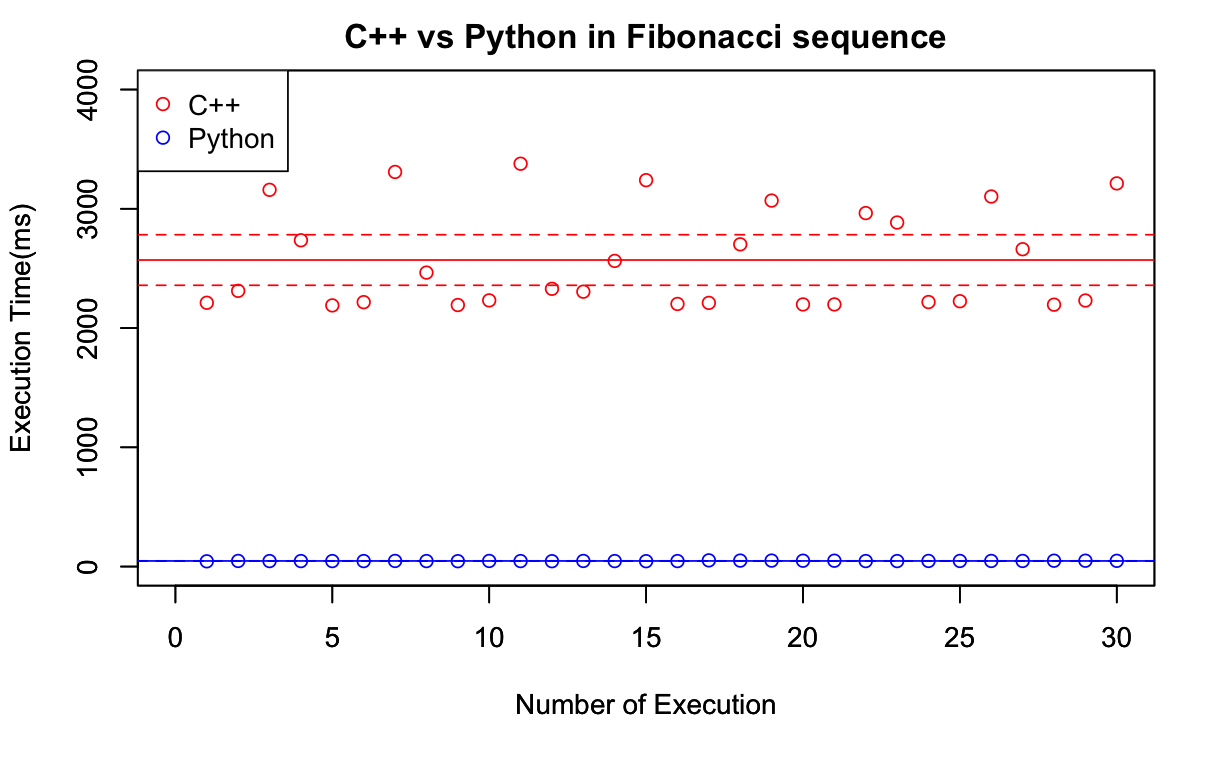
\includegraphics[clip, width=200mm]{00002d.png}
%\caption{Run time in Fibonacci sequence}
%\end{figure}
%
%\begin{figure}[htbp]
%\centering
%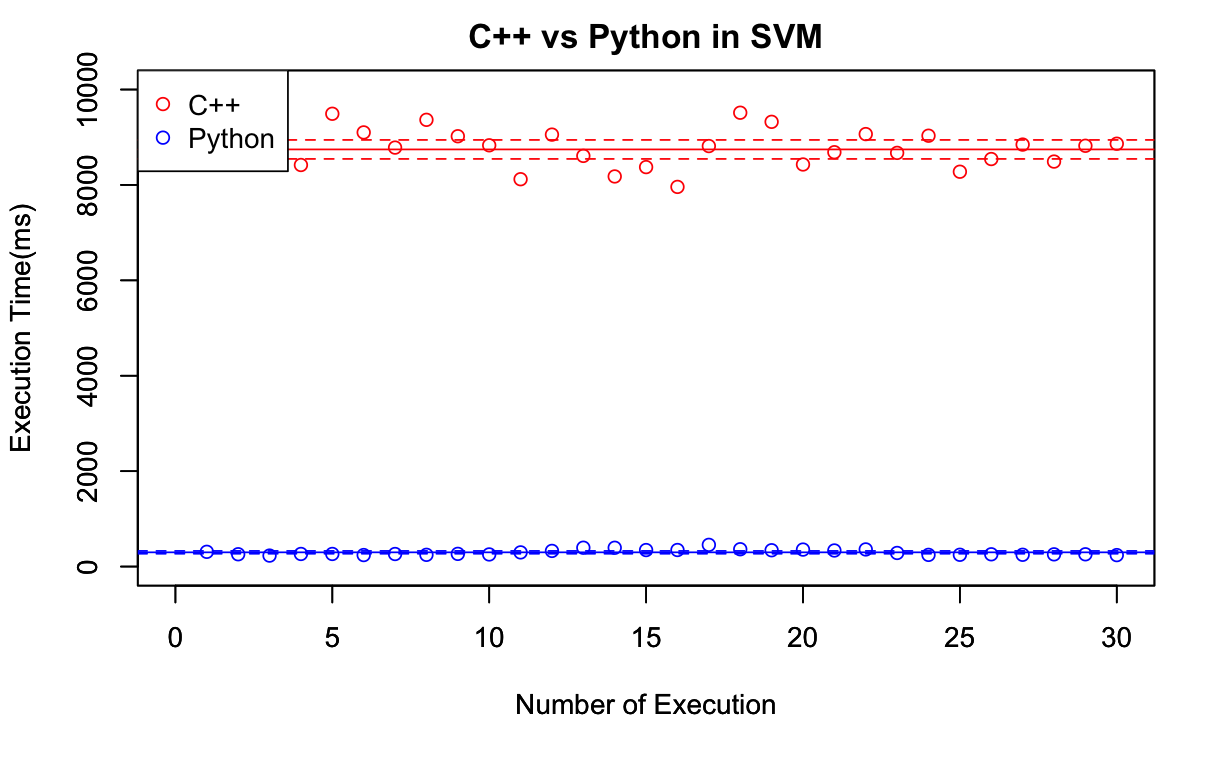
\includegraphics[clip, width=200mm]{000017.png}
%\caption{Run time in SVM}
%\end{figure}

%https://detail.chiebukuro.yahoo.co.jp/qa/question_detail/q11100271691
\begin{figure}[htbp]
\begin{center}
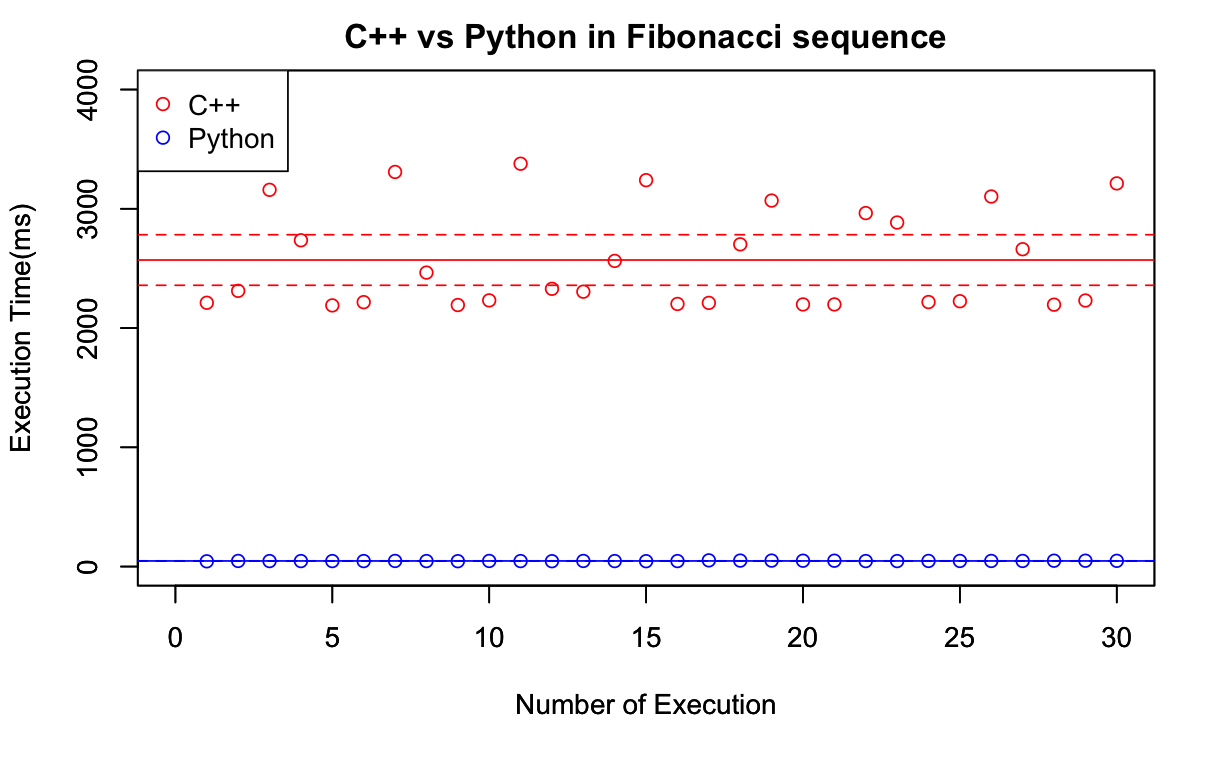
\includegraphics[clip, width=180mm]{00002d.png}
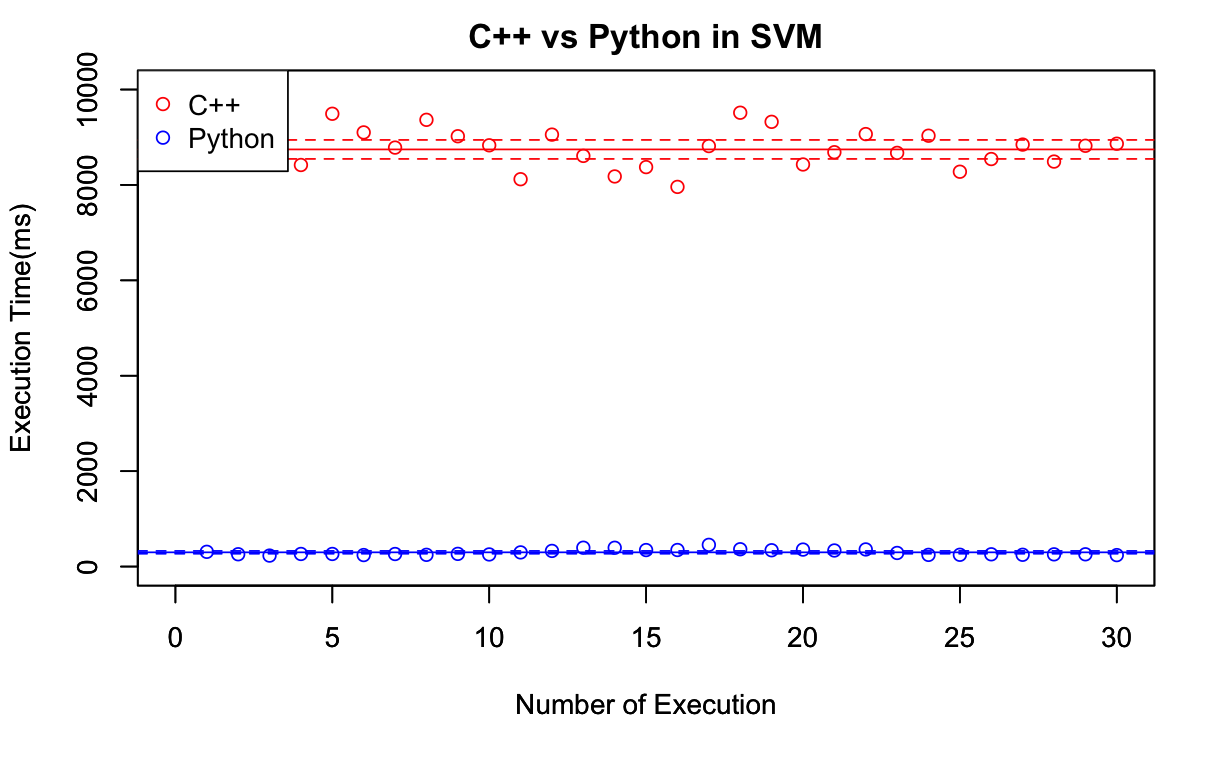
\includegraphics[clip, width=180mm]{000017.png}
\end{center}
\caption{Comparing Run time}
\end{figure}

\section{Conclusion}
\subsection{limitation}
There are many kinds of algorithm. It is almost impossible every single algorithm to implement and measure execution time of it. It would be desirable to test on other environment(e.g., Windows, Linux) not only MacOS. 
\subsection{discussion}
C++ is much faster as I expected. My hypothesis is C++ runs 5 times faster than running in Python. Based on my gathered data and data analysis, C++ runs more than 5 times faster. I need to dig into more wide range of algorithm in the next assignment or propose new hypothesis.
\end{document}